\begin{tikzpicture}[x=.009cm,y=-.009cm,line cap=round,line join=round]
\path[use as bounding box] (15,25) rectangle (860,765);
\draw[line width=.68pt] (114,106)--(830,107);
\draw[line width=.52pt] (114,106)--(112,391);
\draw[line width=.68pt] (112,391)--(817,389);
\draw[line width=.52pt] (114,106)..controls (211,110) and (216,241)..(114,247);
\draw[line width=.52pt] (114,247)..controls (205,254) and (212,379)..(112,391);
\draw[line width=.68pt] (114,530)--(823,532);
\draw[line width=.52pt] (114,530)--(113,739);
\draw[line width=.68pt] (113,739)--(845,742);
\draw[line width=.52pt] (114,530)..controls (165,533) and (184,624)..(114,637);
\draw[line width=.52pt] (114,637)..controls (175,640) and (183,736)..(113,739);
\node[anchor=east,inner sep=0pt,font=\Large] at (97,102) {$i$};
\node[anchor=south,inner sep=0pt,font=\large] at (260,89) {$1+i$};
\node[anchor=east,inner sep=0pt,font=\Large] at (98,248) {$0$};
\node[anchor=center,inner sep=0pt,font=\large\bfseries\itshape] at (549,249) {Raum für $\boldsymbol{t}$ und $\boldsymbol{\dfrac1t}$};
\node[anchor=east,inner sep=0pt,font=\large] at (98,526) {$\dfrac12 i$};
\node[anchor=east,inner sep=0pt,font=\Large] at (98,637) {$0$};
\node[anchor=center,inner sep=0pt,font=\Huge] at (431,663) {$t$};
\end{tikzpicture}
